\chapter{Contexto do Projeto} \label{cap:contexto}

Este capítulo apresenta o contexto real no qual o projeto \textbf{Karaokê Apache} está inserido, incluindo um estudo sobre o segmento de bares com entretenimento musical, índices de digitalização de micro e pequenas empresas no Brasil, análise de ferramentas concorrentes, caracterização do cenário do estabelecimento parceiro, público-alvo, necessidades identificadas e regras de negócio do domínio.

Sistemas de informação permitem às empresas melhorar a eficiência de suas operações e a qualidade do atendimento aos clientes \cite{obrien2013}. No setor de bares e restaurantes, essa informatização já alcança as rotinas comerciais: pesquisa da Abrasel com mais de 1,5 mil empresários indicou que 83\% dos estabelecimentos usam algum software para controlar as vendas e 75\% usam ferramentas de controle financeiro, com espaço de crescimento em outras áreas da operação \cite{jornaldocomercio2023}. Ainda assim, a gestão manual permanece comum entre as micro, pequenas e médias empresas: 39\% delas controlam as despesas com planilhas e cadernos, e 44\% apontam o custo como motivo para não adotar sistemas especializados \cite{folhape2025}. Quando atividades de entretenimento, como noites de karaokê, dependem de controles manuais em papel, o problema operacional chega à experiência do cliente, com pedidos esquecidos, atrasos entre uma apresentação e outra e incerteza sobre a ordem de chamada, como observado no estabelecimento parceiro (Seção \ref{sec:cenario}).

Por outro lado, as principais soluções comerciais de karaokê para estabelecimentos têm custo elevado para um pequeno bar brasileiro e não utilizam o acervo do YouTube. Plataformas internacionais como o \textbf{Singa Business} \cite{singa2026} e o \textbf{KaraFun Business} \cite{karafun2026} cobram mensalidades em dólar: os planos do KaraFun Stage, voltados a apresentações com cantores, custam de US\$ 49,99 a US\$ 209,99 por mês, com compromisso de 12 meses \cite{karafunstage2026}, e os do Singa Business partem de US\$ 59 por mês \cite{singablog2026}. Ambas trabalham com catálogos próprios licenciados, com mais de 90 mil músicas no KaraFun e mais de 140 mil no Singa \cite{karafun2026,singablog2026}, o que impede o uso de versões de karaokê disponíveis no YouTube. Já o \textbf{Juks} apresenta-se como uma \textit{jukebox} digital para bares e restaurantes \cite{juks2026}, voltada à execução de músicas no ambiente, e não à organização de apresentações de karaokê. A Tabela \ref{tab:concorrencia} sintetiza o estudo comparativo realizado pela equipe.

\begin{table}[H]
\IBGEtab{%
  \caption{Estudo comparativo entre soluções existentes no mercado e o sistema proposto.}%
  \label{tab:concorrencia}%
}{%
  \footnotesize
  \begin{tabularx}{\textwidth}{Xcccc}
    \toprule
    \textbf{Critério / Recurso Analisado} & \textbf{Singa Business} & \textbf{KaraFun Business} & \textbf{Juks} & \textbf{Karaokê Apache} \\
    \midrule
    Pedidos pelo celular via QR Code no telão & Parcial & Sim & Sim & Sim \\
    Escolha de vídeos pelo próprio sistema & Sim & Sim & Sim & Sim \\
    Fila de cantores com moderação de palco & Sim & Sim & Não & Sim \\
    Reprodutor dedicado para o telão (TV) & Sim & Sim & Parcial & Sim (Electron) \\
    Suporte ao acervo de karaokê do YouTube & Não & Não & Parcial & Sim \\
    Bloqueio automático de música duplicada & Parcial & Parcial & Sim & Sim \\
    Custo para o bar parceiro & Alto (US\$) & Alto (US\$) & Médio (R\$) & \begin{tabular}[t]{@{}c@{}}Baixo (somente\\hospedagem)\end{tabular} \\
    \bottomrule
  \end{tabularx}%
}{%
  \fonte{Elaborado pelos autores a partir de \citeonline{karafunstage2026}, \citeonline{singablog2026} e \citeonline{juks2026}.}%
}
\end{table}

\section{Cenário} \label{sec:cenario}

O parceiro demandante do projeto é o estabelecimento comercial \textbf{Apache Gru Rock Bar}, registrado sob a razão social \texttt{APACHE GRU ROCK BAR LTDA} e inscrito no CNPJ sob o n{\textordmasculine} \texttt{64.687.141/0001-07}. O bar está localizado na Avenida Torres Tibagy, n{\textordmasculine} 58, no bairro Gopouva, em Guarulhos -- SP (CEP 07062-000), e sua atividade principal é classificada no CNAE 5611-2/05, que corresponde a bares e outros estabelecimentos especializados em servir bebidas, com entretenimento \cite{cnpjapi2026}.

O Apache Gru é um bar de rock que recebe apresentações de bandas, como os shows do tributo \textit{Roots -- Sepultura Tributo} realizados em agosto de 2025 e janeiro de 2026 \cite{setlistfm2026}. Às quintas-feiras, a partir das 20h, o bar realiza a sua \textbf{Noite de Karaokê}, sem cobrança para cantar \cite{motofest2026}. No cenário atual de operação do salão, é utilizado um projetor \textit{whitelabel} com conexão à internet, sendo diretamente por ele acessado o aplicativo do YouTube e colocados os vídeos manualmente a cada apresentação.

Dessa forma, a dinâmica da Noite de Karaokê ocorria de maneira inteiramente manual: os clientes precisavam solicitar suas músicas verbalmente ou em anotações de papel, e o organizador precisava digitar e pesquisar manualmente cada vídeo no YouTube diretamente pela interface do projetor \textit{whitelabel} conectado à internet, interrompendo a fluidez entre uma apresentação e outra e dificultando o controle da fila de espera.

\section{Público-Alvo}

O projeto atende diretamente três perfis de público-alvo envolvidos na operação da Noite de Karaokê do Apache Gru Rock Bar:

\begin{enumerate}
  \item \textbf{Frequentadores e Cantores Amadores (Clientes do Bar):} jovens e adultos frequentadores do Apache Gru Rock Bar que comparecem individualmente ou em grupos de amigos. Possuem familiaridade cotidiana com smartphones e aplicativos web, mas buscam uma interação rápida e intuitiva em ambiente noturno (baixa luminosidade), sem desejar baixar aplicativos pesados apenas para pedir uma música;
  \item \textbf{Organizador / Operador de Palco e Som (Administrador Operacional):} colaborador responsável por conduzir a noite de karaokê, chamar o próximo cantor no microfone, controlar o equipamento de áudio e garantir que o telão exiba continuamente a música correta sem interrupções técnicas;
  \item \textbf{Gestores e Proprietários do Estabelecimento:} responsáveis pela administração do Apache Gru Rock Bar, interessados em aumentar a satisfação e o tempo de permanência dos clientes no salão, reduzir a sobrecarga da equipe de atendimento e conhecer o repertório mais popular entre seus frequentadores.
\end{enumerate}

\section{Necessidades Identificadas}

A partir do acompanhamento do cenário operacional do Apache Gru Rock Bar e das conversas com os envolvidos, foram identificadas quatro necessidades fundamentais da comunidade atendida:

\begin{itemize}
  \item \textbf{N01 -- Autonomia para escolha de vídeos pelo próprio sistema:} necessidade de permitir que o cliente acesse a plataforma via QR Code exibido no telão e escolha o vídeo musical desejado diretamente pelo próprio sistema em seu celular, eliminando o uso de fichas de papel;
  \item \textbf{N02 -- Transparência e previsibilidade na fila de espera:} necessidade de dar visibilidade pública e em tempo real para todos os participantes sobre qual música está tocando no momento, quantas pessoas estão na fila e qual é a ordem das próximas apresentações;
  \item \textbf{N03 -- Prevenção de repetições e garantia de rotatividade justa:} necessidade de evitar que uma mesma canção seja cantada repetidas vezes em curto espaço de tempo ou que um único participante monopolize a fila;
  \item \textbf{N04 -- Automação e limpeza visual da reprodução no telão:} necessidade de substituir a busca manual direta no projetor \textit{whitelabel} por um reprodutor dedicado, controlado remotamente a partir da fila, que exiba no telão o vídeo da música da vez sem expor telas de busca ou menus intermediários.
\end{itemize}

\section{Regras de Negócio}

Para atender às necessidades identificadas respeitando as políticas operacionais do estabelecimento, foram estabelecidas cinco Regras de Negócio (RN00 a RN04) em nível conceitual, documentadas na planilha de engenharia do projeto (\textit{Regras de Negócio | Requisitos -- Separados por Componentes}) e descritas na Tabela \ref{tab:regras_negocio}.

\begin{table}[H]
\IBGEtab{%
  \caption{Regras de negócio do domínio do sistema Karaokê Apache.}%
  \label{tab:regras_negocio}%
}{%
  \footnotesize
  \begin{tabularx}{\textwidth}{p{1.4cm}p{3.4cm}X}
    \toprule
    \textbf{Código} & \textbf{Regra de Negócio} & \textbf{Descrição Conceitual e Política de Domínio} \\
    \midrule
    RN00 & Validação de Disponibilidade da Música & Toda solicitação musical deve referenciar um item disponível no catálogo ou uma fonte audiovisual válida e ativa antes de ingressar na fila de apresentações. \\
    \addlinespace
    RN01 & Proibição de Música Duplicada na Fila Ativa & Uma música que já se encontra aguardando execução na fila ativa ou que está sendo reproduzida no momento não pode ser novamente inserida na fila até a conclusão de sua execução atual. \\
    \addlinespace
    RN02 & Limite de Pedidos Simultâneos por Participante & Para preservar a rotatividade entre as mesas do bar, cada cliente, identificado como visitante ou por sua conta, possui um limite configurável de pedidos ativos simultâneos na fila (padrão de 1 a 2 músicas pendentes por vez). \\
    \addlinespace
    RN03 & Exclusividade Administrativa do Controle de Palco & O acionamento de início da reprodução, o avanço para a próxima faixa e a remoção de itens da fila (inclusive por ausência do cantor) são prerrogativas exclusivas do organizador (Administrador). A ordem da fila segue a ordem de chegada dos pedidos (FIFO) e não é alterada manualmente. \\
    \addlinespace
    RN04 & Ciclo de Vida e Rastreabilidade do Pedido & Todo pedido aceito percorre um fluxo controlado de estados (\textit{Na Fila}, \textit{Reproduzindo}, \textit{Concluído} ou \textit{Cancelado}), mantendo o registro do solicitante e do horário para controle da sessão. \\
    \bottomrule
  \end{tabularx}%
}{%
  \fonte{Elaborado pelos autores a partir da planilha de engenharia do projeto (2026).}%
}
\end{table}

A Figura \ref{fig:atividades} apresenta o \textbf{Diagrama de Atividades UML} que modela o fluxo operacional de negócio desde a solicitação da música pelo cliente na mesa até a conclusão da apresentação no palco, destacando os pontos de decisão regidos pelas regras RN00, RN01, RN02 e RN03.

\Needspace{20cm}
\begin{figure}[H]
  \caption{Diagrama de Atividades UML -- Fluxo de Pedido Musical e Execução na Fila}
  \label{fig:atividades}
\begin{center}
  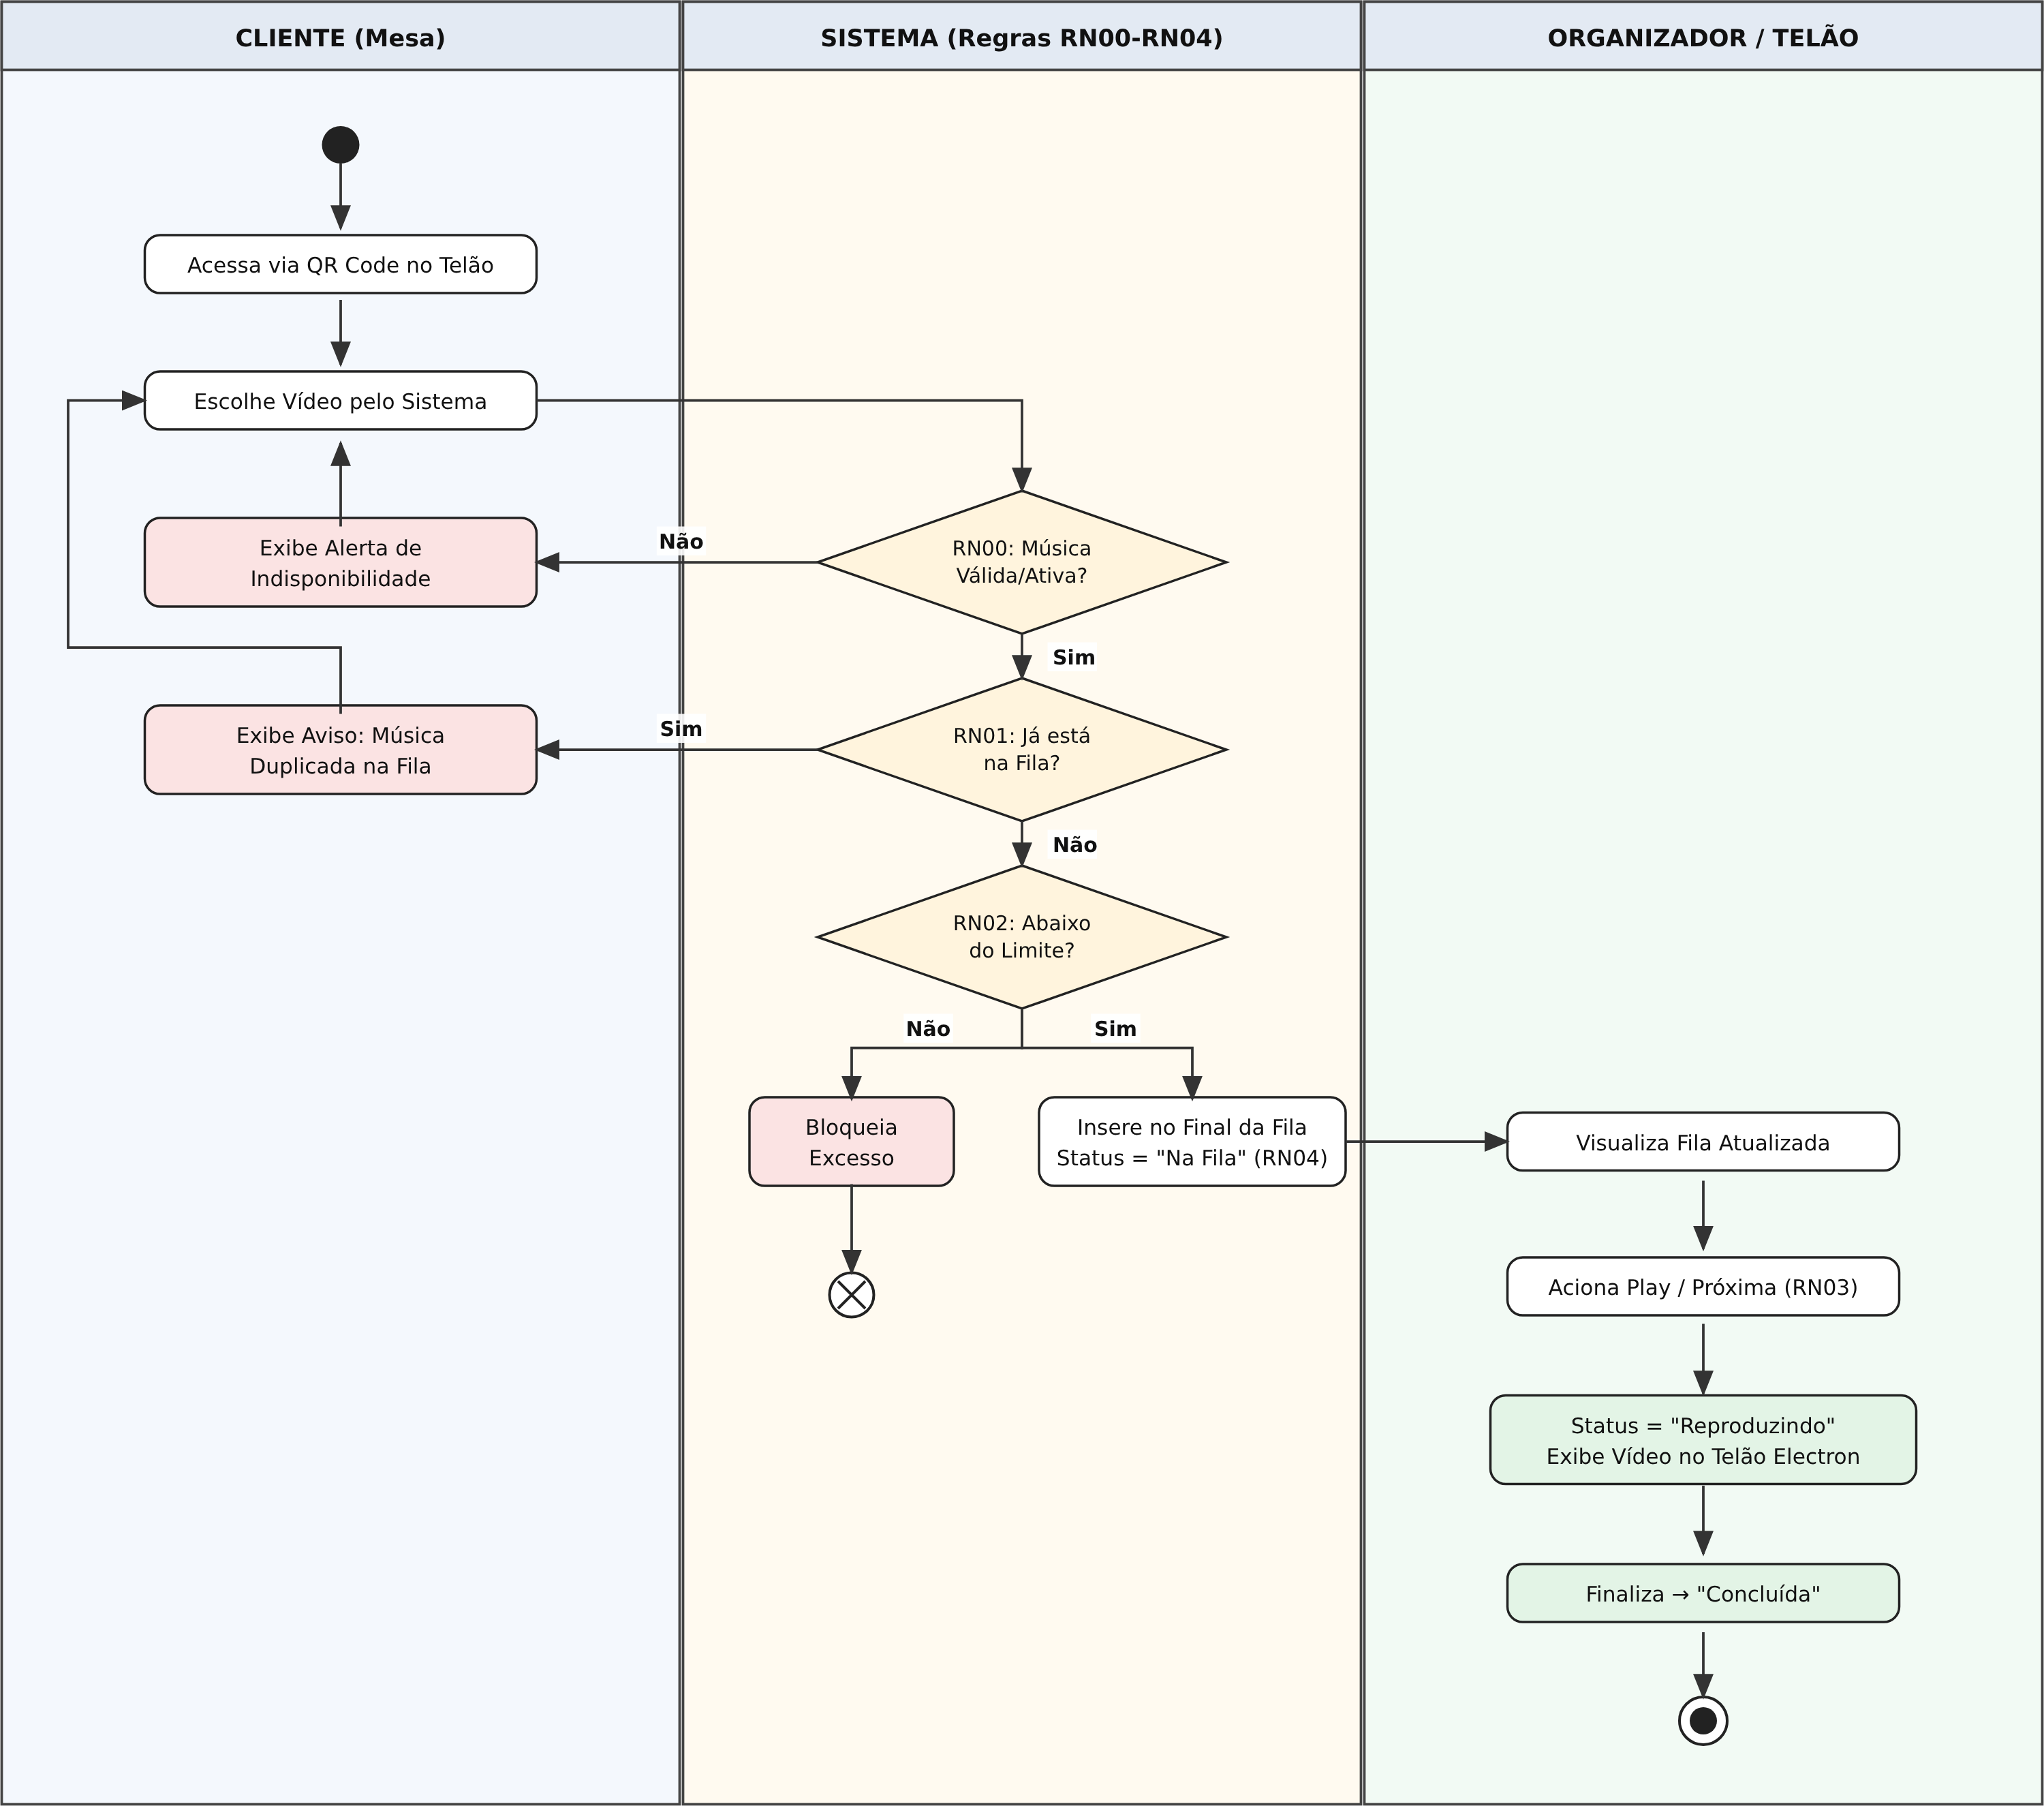
\includegraphics[width=0.95\textwidth,height=0.78\textheight,keepaspectratio]{imagens/diagrama_atividades.png}
\end{center}
\legend{Fonte: Elaborado pelos autores (2026).}
\end{figure}

%% -------------------------------------------------------------------------- %%
